\subsection{Design}
This section describes the main aspects of the VFS Browser applicatoin. It shows
the implementation of the core interfaces and classes.

\subsubsection{GUI classes}\label{sec:guiClasses}
Figure \ref{fig:gui_classes} gives an overview of the main interfaces and
classes that were implemented for the gui. The implementation followed the rules
of a MVC design dividing the aspects of Model View and Control to their
respective classes. According to the partition of MVC the classes were
partitioned into the packages \textit{model, view and controller}.

\begin{figure}[h!]
\centering
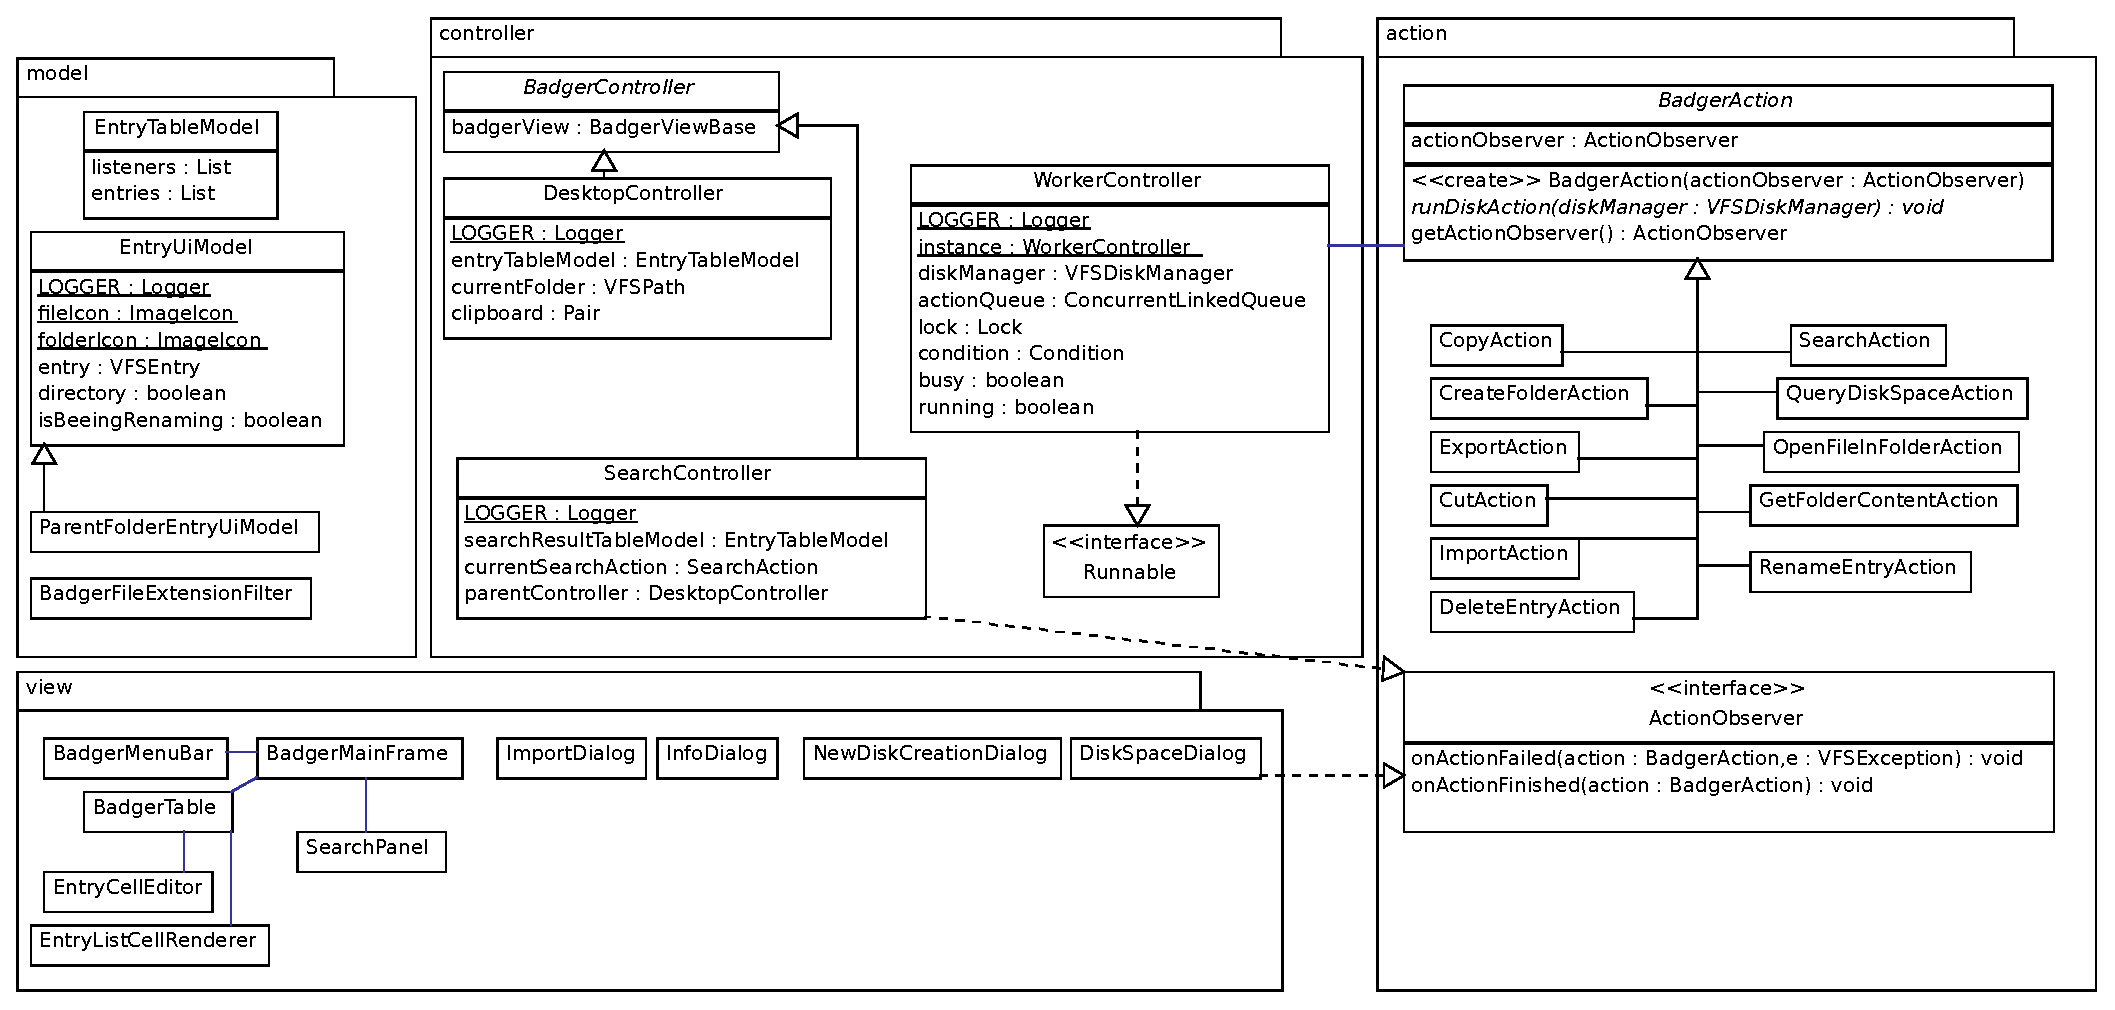
\includegraphics[width=1\textwidth]{figures/gui_classes.eps}
\caption{gui classes}
\label{fig:gui_classes}
\end{figure}


\subsubsection{Decoupling of GUI and working threads}
This section describes the way how the decoupling from GUI and working threads
was implemented. This decoupling mades the GUI still responsive even tough some
long running tasks like import or search would be running. Figure
\ref{fig:decouple_threads} shows the sequence diagram of the example ``Import'':
The \textit{DesktopController} which lives in the GUI thread creates a new
\textit{ImportAction} that is enqueued in the \textit{WorkerController}'s action queue. It is worth to mention, that the
\textit{WorkerController} is a singleton, that has an \textit{instance} field. The
\textit{WorkerController} has a thread that works on a blocking queue and every
time it gets a \textit{BadgerAction} the thread wakes up and performs the action
on the VFS core API. After the API work is done (in this case the import of
files), the \textit{WorkerController} calls the corresponding
\textit{ActionObserver}, which is in most cases the \textit{DesktopController}
instance, so that the GUI can be updated. This design ensures single threaded
access on the VFS core API with keeping the GUI responsive.

\begin{figure}[h!]
\centering
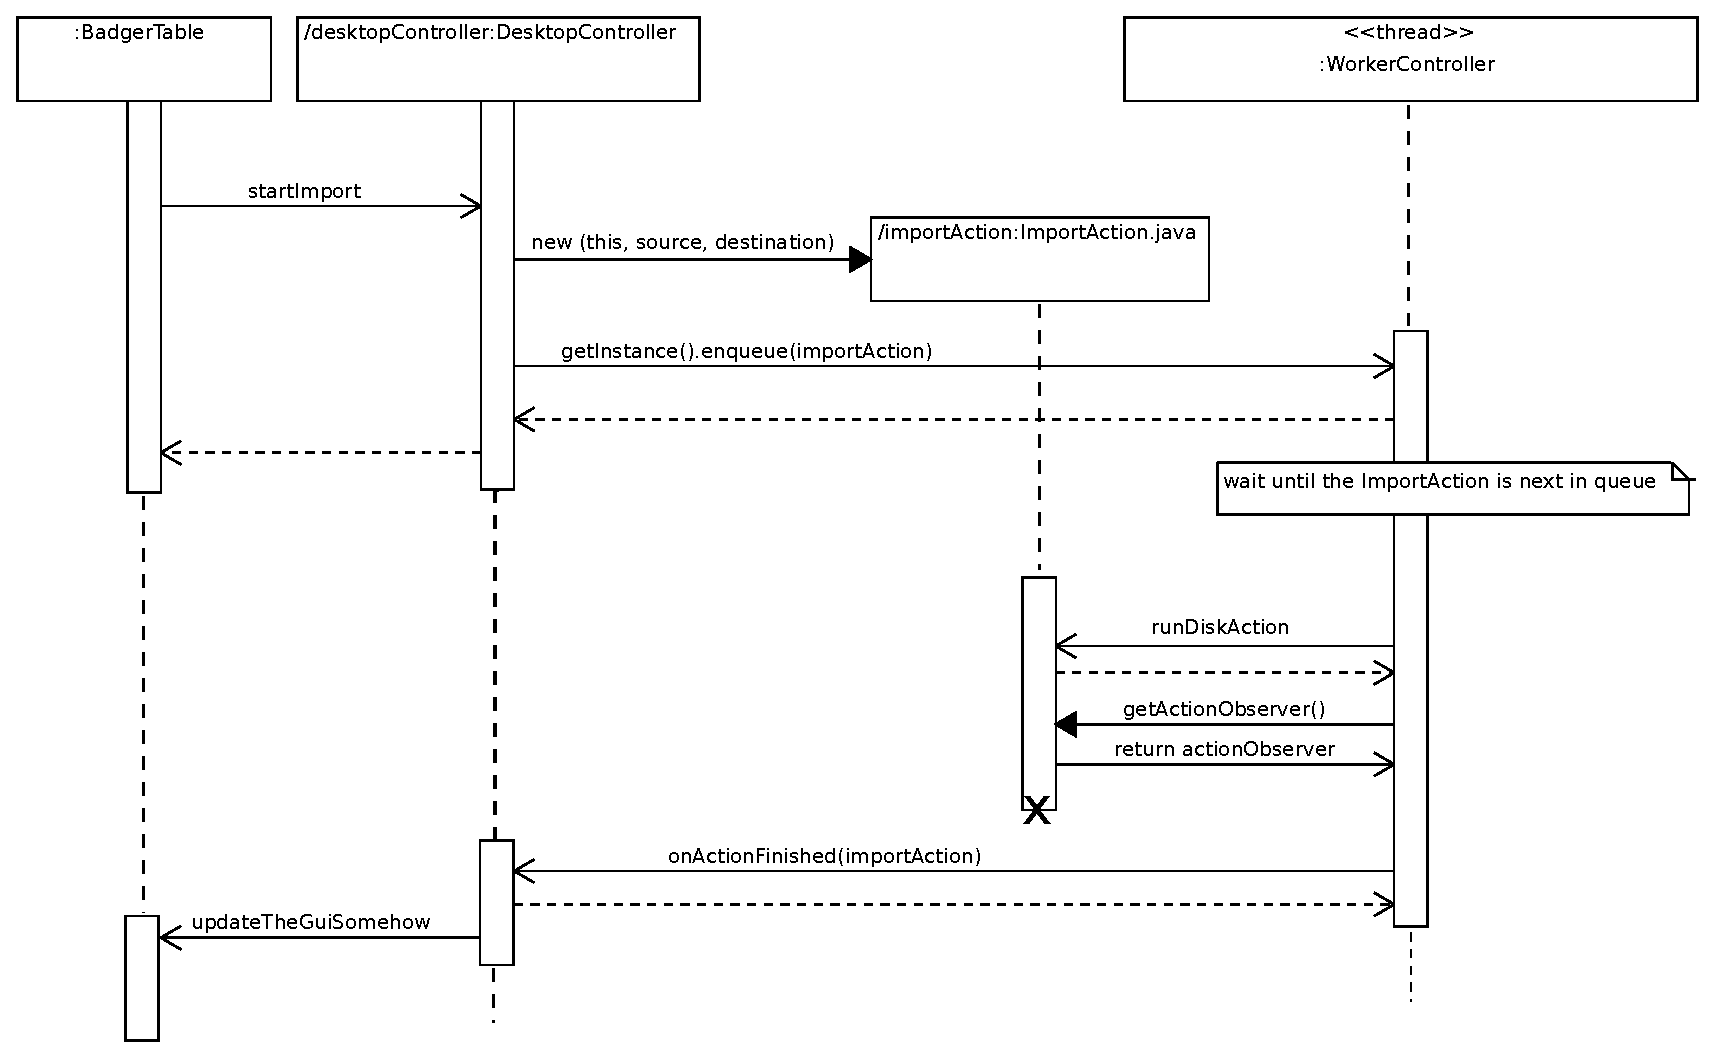
\includegraphics[width=1\textwidth]{figures/single_threaded_access.eps}
\caption{example of decoupling import from gui}
\label{fig:decouple_threads}
\end{figure}

Even when doing a seach the decoupling works pretty well: The
\textit{SearchAction} uses the VFS cores \textit{FindInFolderCallback} to update
the \textit{SearchController} which lives in the GUI thread every time finds an
entry.

\subsubsection{Search}
Searching files can be done in a separate Panel: After entering the search
string one is allowed to switch several flags like ``case sensitive'' or
``search subfolder'' and one can change the search folder.


\subsubsection{Keyboard and Mouse support}

\paragraph{Keyboard Shortcuts}
\paragraph{Drag \& Drop}